\section{Introduction}
In the \emph{Introduction to SystemVerilog} step, I had the opportunity to tackle the limitations of the directed testing approach, getting familiar with some common principles of more advanced verification methodologies and their elected language, \sv. Primarily guided by~\cite{spear:svfe}, I applied object-oriented and generic programming principles to craft a reusable, templated testbench framework that I could specialize for specific \acs{dut}s. Through the design and development of the entire testbench architecture, I gained a better understanding of the techniques that go into the classes and utilities of the \uvm library, which established itself as a de facto industry standard for functional verification.

\subsection{The \acl{uvm}}
The complexity of digital designs continues to escalate, posing tough challenges to ensure their correctness and reliability. Curated by the Accelera \uvm Working Group, this methodology focuses on establishing modularity, scalability, and reusability in verification environments, with the core objective of augmenting design productivity.
Both the standard~\cite{IEEE:1800.22020} and the class library are available free of charge; the library is conveniently shipped in the package \svinline{uvm_pkg}.

\subsubsection{Base Classes: An Overview}
The basic building blocks for all environments are components and the transactions they use to communicate.
\begin{itemize}
    \item All components and transactions derive from \svinline{uvm_object}, an abstract base class whose primary role is to define an interface for common operations as \svinline{create}, \svinline{copy}, and \svinline{compare}. It also defines interfaces for instance identification, which includes name, type name, id, and seeding.
    \item Components are objects derived from \svinline{uvm_component} that exist throughout the simulation. They establish a structural hierarchy, like modules and program blocks, and take part in the execution under the control of a central phasing mechanism; for each phase, they define a callback function or task that is executed in a precise order.
    \item Unlike components, transactions are transient in nature. In the simpler cases, they can be derived directly from \svinline{uvm_transaction}, but for operating in the sequence mechanism, the base class is \svinline{uvm_sequence_item}.
\end{itemize}

\subsubsection{The \acs{uvm} Architecture}\label{subsubsec:uvm_arch}

\begin{figure}
    \centering
    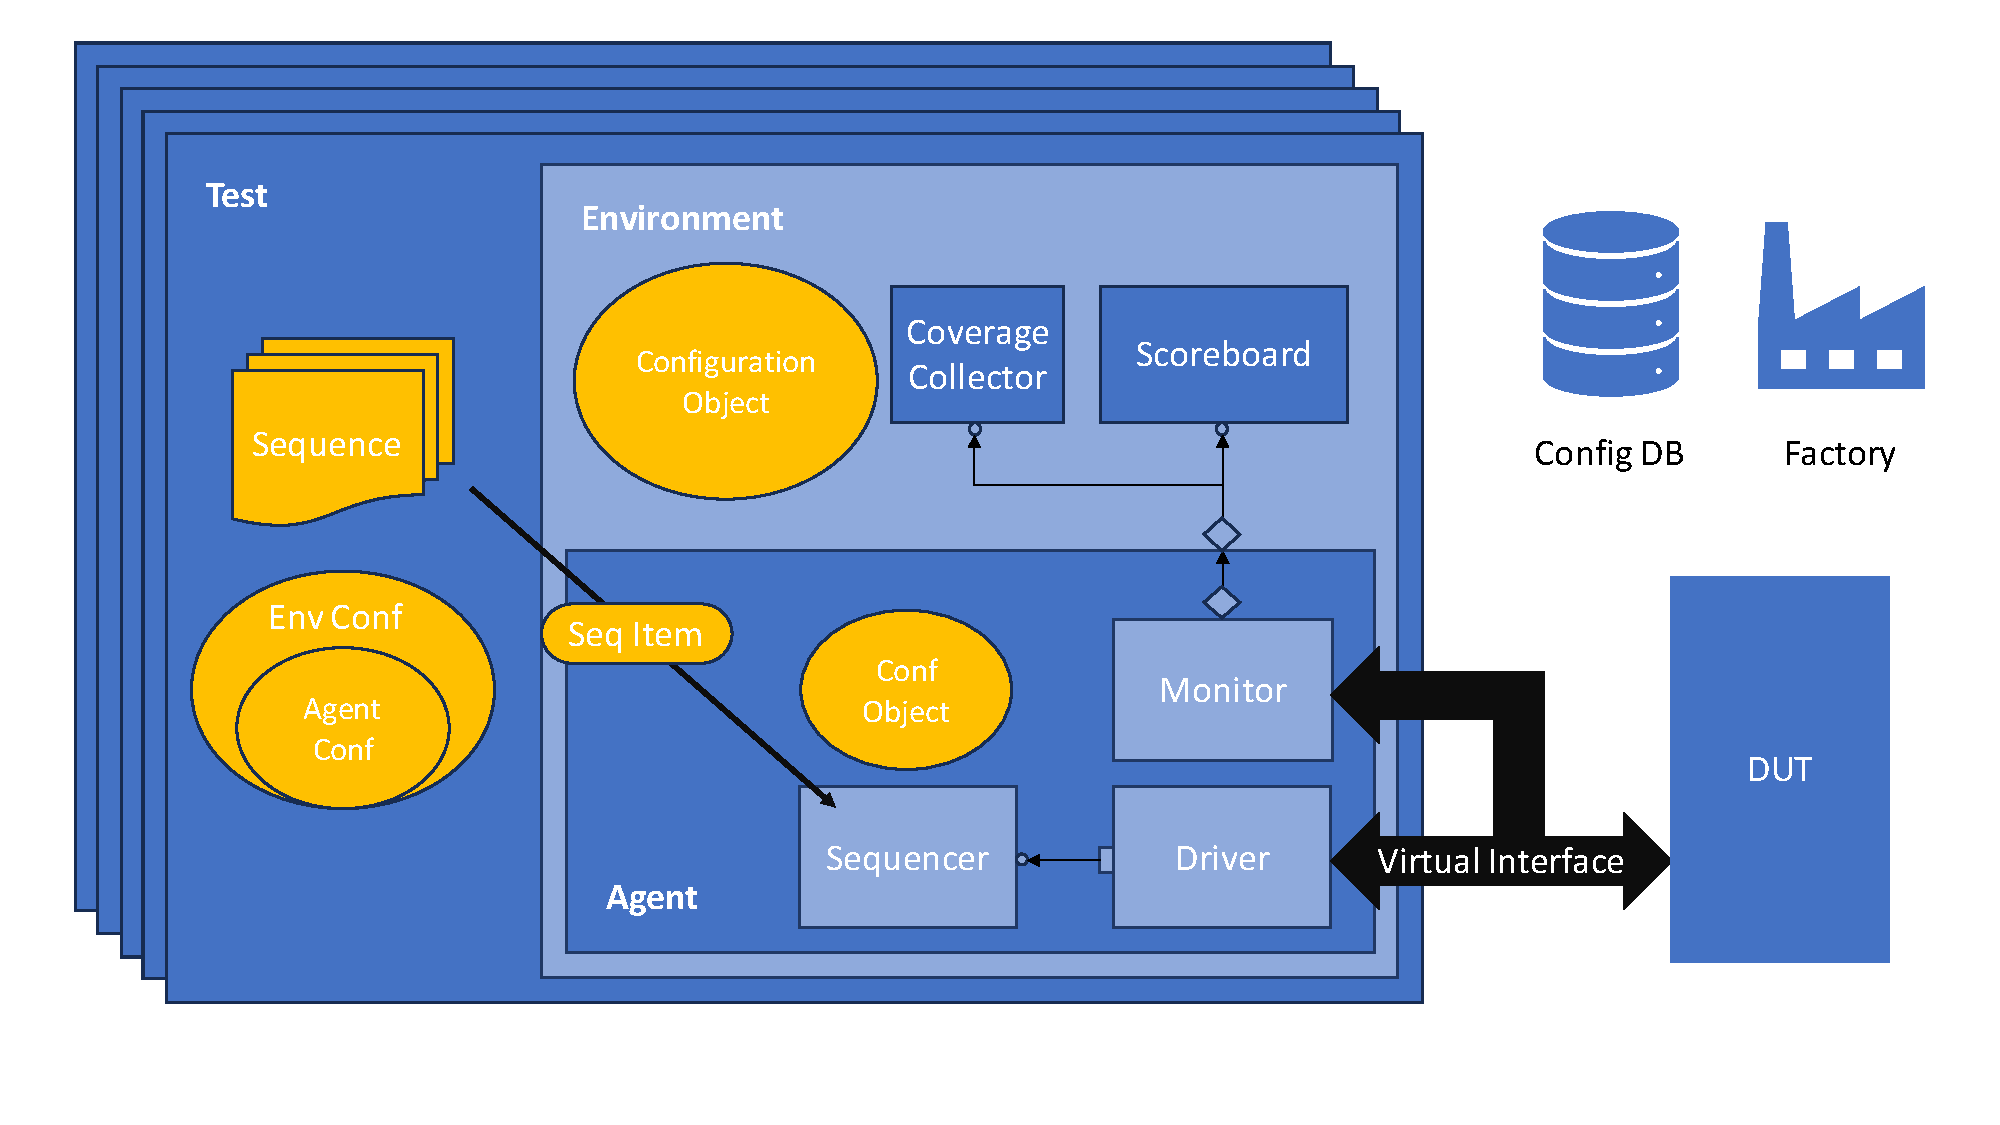
\includegraphics[width=\linewidth]{fig/uvm_architecture.pdf}
    \caption{Typical \acs{uvm}-based testbench architecture. Each interface of the \acs{dut} is served by an agent: both the driver and the monitor communicate at the signal level, whereas any other communication is at the transaction level. A library of test components can use the same environment, possibly customizing it via factory overrides and the configuration database.}
    \label{fig:generic-uvm-arch}
\end{figure}

The typical architecture of a \uvm-based testbench is shown in~\cref{fig:generic-uvm-arch}. For each interface of the \dut there is a dedicated verification component called agent, which includes:
\begin{itemize}
    \item The driver, whose job is to communicate at the signal level with the \dut through the interface, translating incoming sequence items to pin wiggles.
    \item The sequencer, which arbitrates the flow of sequence items to the driver, possibly routing its responses back to the correct generator sequence. On a given sequencer it's possible to have multiple sequences executing, which is why it supports arbitration. Sequences are objects whose job is to generate a stream of sequence items.
    \item The monitor, which recognizes the pin-level activity on the interface and turns it into transactions that get broadcasted to other environment components through an analysis port.
    \item A configuration object, which contains all the information the agent needs to know how to operate; for instance, the virtual interface handle.
\end{itemize}
The environment acts as a container of interrelated verification components; it gets its configuration object first and uses it to configure itself and the components it instantiates. Typically, these additional blocks include a coverage collector, which tracks progress in the verification plan, and the scoreboard, which checks \dut responses to the randomized stimulus. In turn, the environment is instantiated by a test component: it specifies the sequences to execute and the customization of the environment both in terms of factory overrides and configuration objects stored in the database. It is common to develop a base test class and craft a library of extended tests that only add sequences and stimulus-specific customizations.

\subsection{The Hands-On Experience}\label{subsec:handson}

\begin{listing}
\begin{minted}[bgcolor=backcolor, fontsize=\scriptsize]{vhdl}
entity p4_adder is
  generic (
    nbit:           integer := 32;
    nbit_per_block: integer := 4);
  port (
    a:    in    std_logic_vector(nbit-1 downto 0);
    b:    in    std_logic_vector(nbit-1 downto 0);
    cin:  in    std_logic;
    s:    out   std_logic_vector(nbit-1 downto 0);
    cout: out   std_logic
  );
end entity;
\end{minted}
\caption{\vhdl interface of Intel's Pentium IV adder under test.}
\label{list:dut_p4}
\end{listing}

\begin{listing}
\begin{minted}[bgcolor=backcolor, fontsize=\scriptsize]{vhdl}
entity windowed_rf is
  generic (
    M:          positive := 8;  -- number of global registers
    N:          positive := 8;  -- number of registers per register subset 
    F:          positive := 8;  -- number of register sets (N "in" + N "local")
    width_data: positive := 64  -- parallelism of data
  );
  port (
    clk:      in  std_logic;
    reset:    in  std_logic;  -- synchronous, write-through
    enable:   in  std_logic;  -- gates rd1, rd2, wr

    -- 2R / 1W ports 
    rd1:      in  std_logic;  -- enables synchronous reading on port R1
    rd2:      in  std_logic;  -- enables synchronous reading on port R2
    wr:       in  std_logic;  -- enables synchronous writing

    -- Addressing convention:
    -- Windowed Register Address  Register Address
    --   in[0] - in[N-1]            r[M+2*N] - r[M+3*N-1]
    --   local[0] - local[N-1]      r[M+N] - r[M+2*N-1]
    --   out[0] - out[N-1]          r[M] - r[M+N-1]
    --   global[0] - global[M-1]    r[0] - r[M-1]

    add_rd1:  in  std_logic_vector(clog2(M+3*N)-1 downto 0);
    add_rd2:  in  std_logic_vector(clog2(M+3*N)-1 downto 0);
    add_wr:   in  std_logic_vector(clog2(M+3*N)-1 downto 0);

    datain:   in  std_logic_vector(width_data-1 downto 0);
    out1:     out std_logic_vector(width_data-1 downto 0);
    out2:     out std_logic_vector(width_data-1 downto 0);

    -- execution flow control
    call:     in  std_logic;  -- subroutine call
    ret:      in  std_logic;  -- subroutine return
    bypass:   out std_logic;  -- '0' when available for external operations

    -- interface to memory management unit
    fill:     out std_logic;
    spill:    out std_logic;

    mmu_done: in  std_logic;  -- fill/spill synchronization
    mmu_data: in  std_logic_vector(width_data-1 downto 0)
  );
end entity;
\end{minted}
\caption{\vhdl interface of the fixed-size windowed register file under test.}
\label{list:dut_wrf}
\end{listing}

\begin{sidewaysfigure}
    \centering
    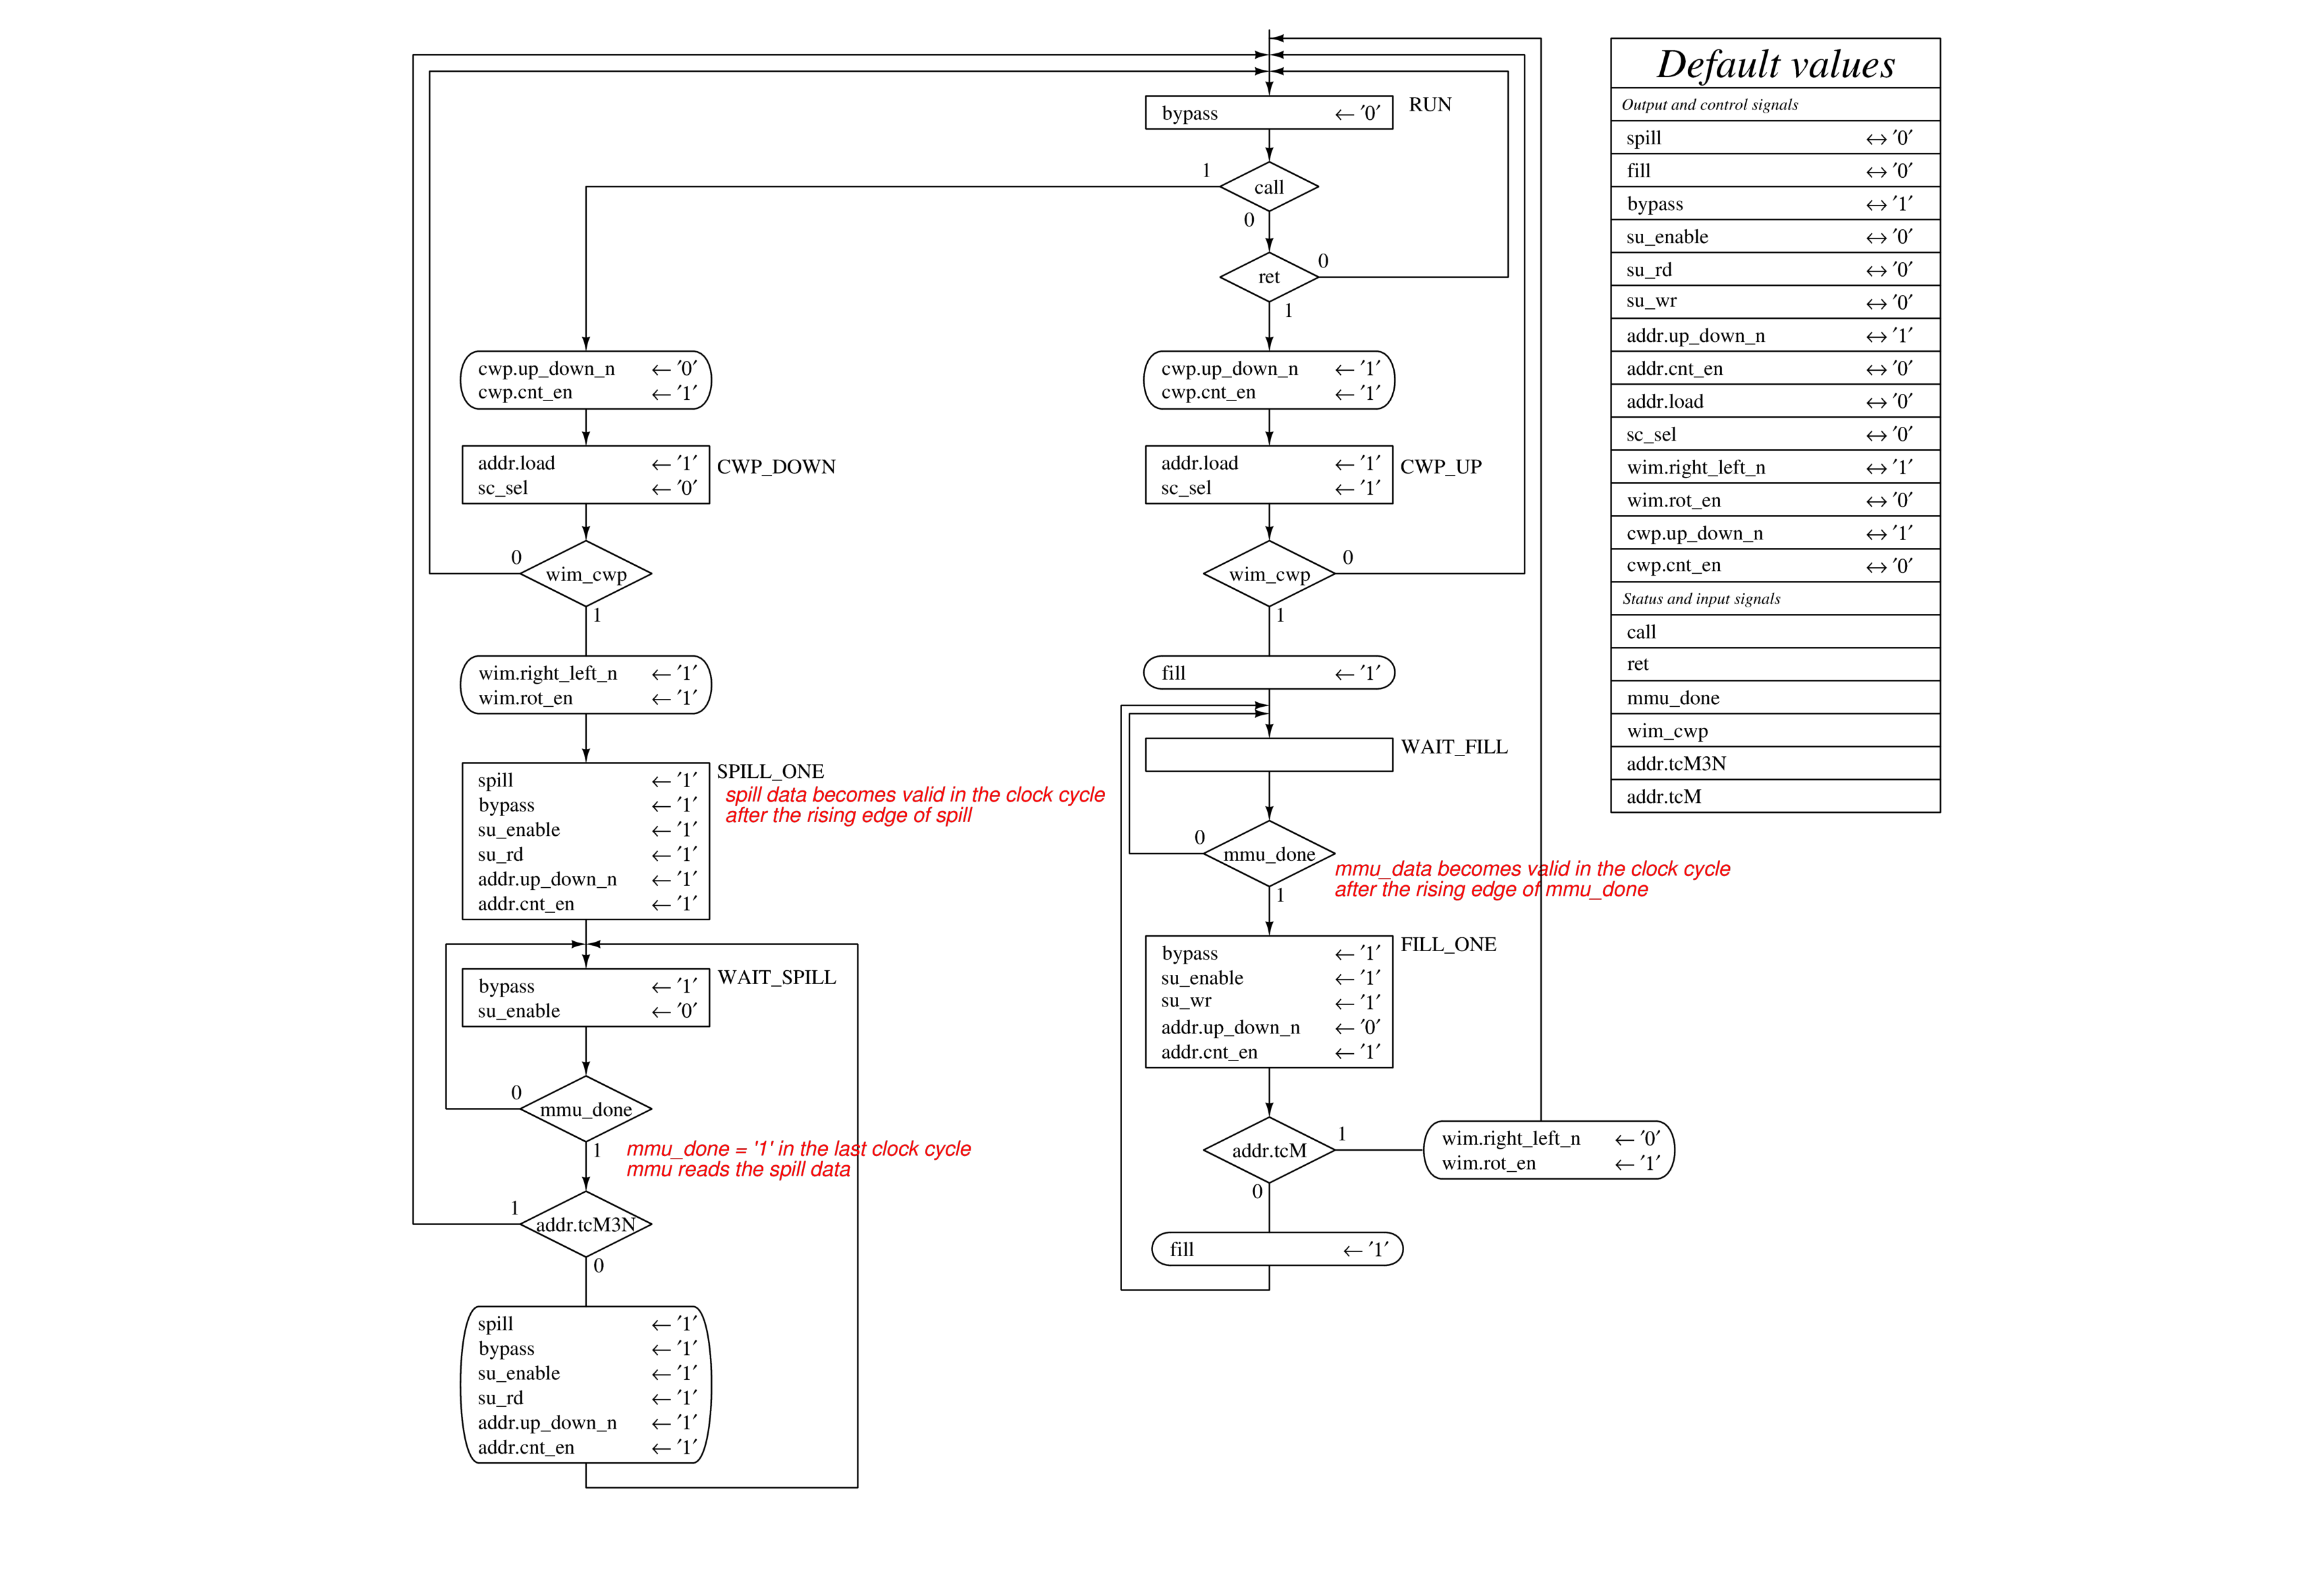
\includegraphics[width=\textwidth]{fig/windowed_rf/windowed_rf_cu.pdf}
    \caption{Windowed register file \acs{asm} chart, describing the signal-level details of managing call and return requests. When both the \vhdlinline{call} and \vhdlinline{ret} signals are asserted, the call request takes precedence. In both cases, the \vhdlinline{bypass} signal is raised while the register file is busy. If the request triggers a spill or fill operation, the \svinline{spill} signal is raised with a one-cycle delay after the \vhdlinline{bypass} signal, whereas the \vhdlinline{fill} signal is raised within the same cycle. The memory management unit must set the \vhdlinline{mmu_done} signal according to specifications: in the last clock cycle it reads data on \vhdlinline{out1} for a spill operation; in the clock cycle before the data on \vhdlinline{mmu_data} becomes valid for a fill operation.}
    \label{fig:wrf_asm}
\end{sidewaysfigure}

\begin{figure}
    \vspace*{-2.5\baselineskip}
    \begin{adjustwidth}{-1cm}{-1cm}
    \thisfloatpagestyle{empty}
    \centering
    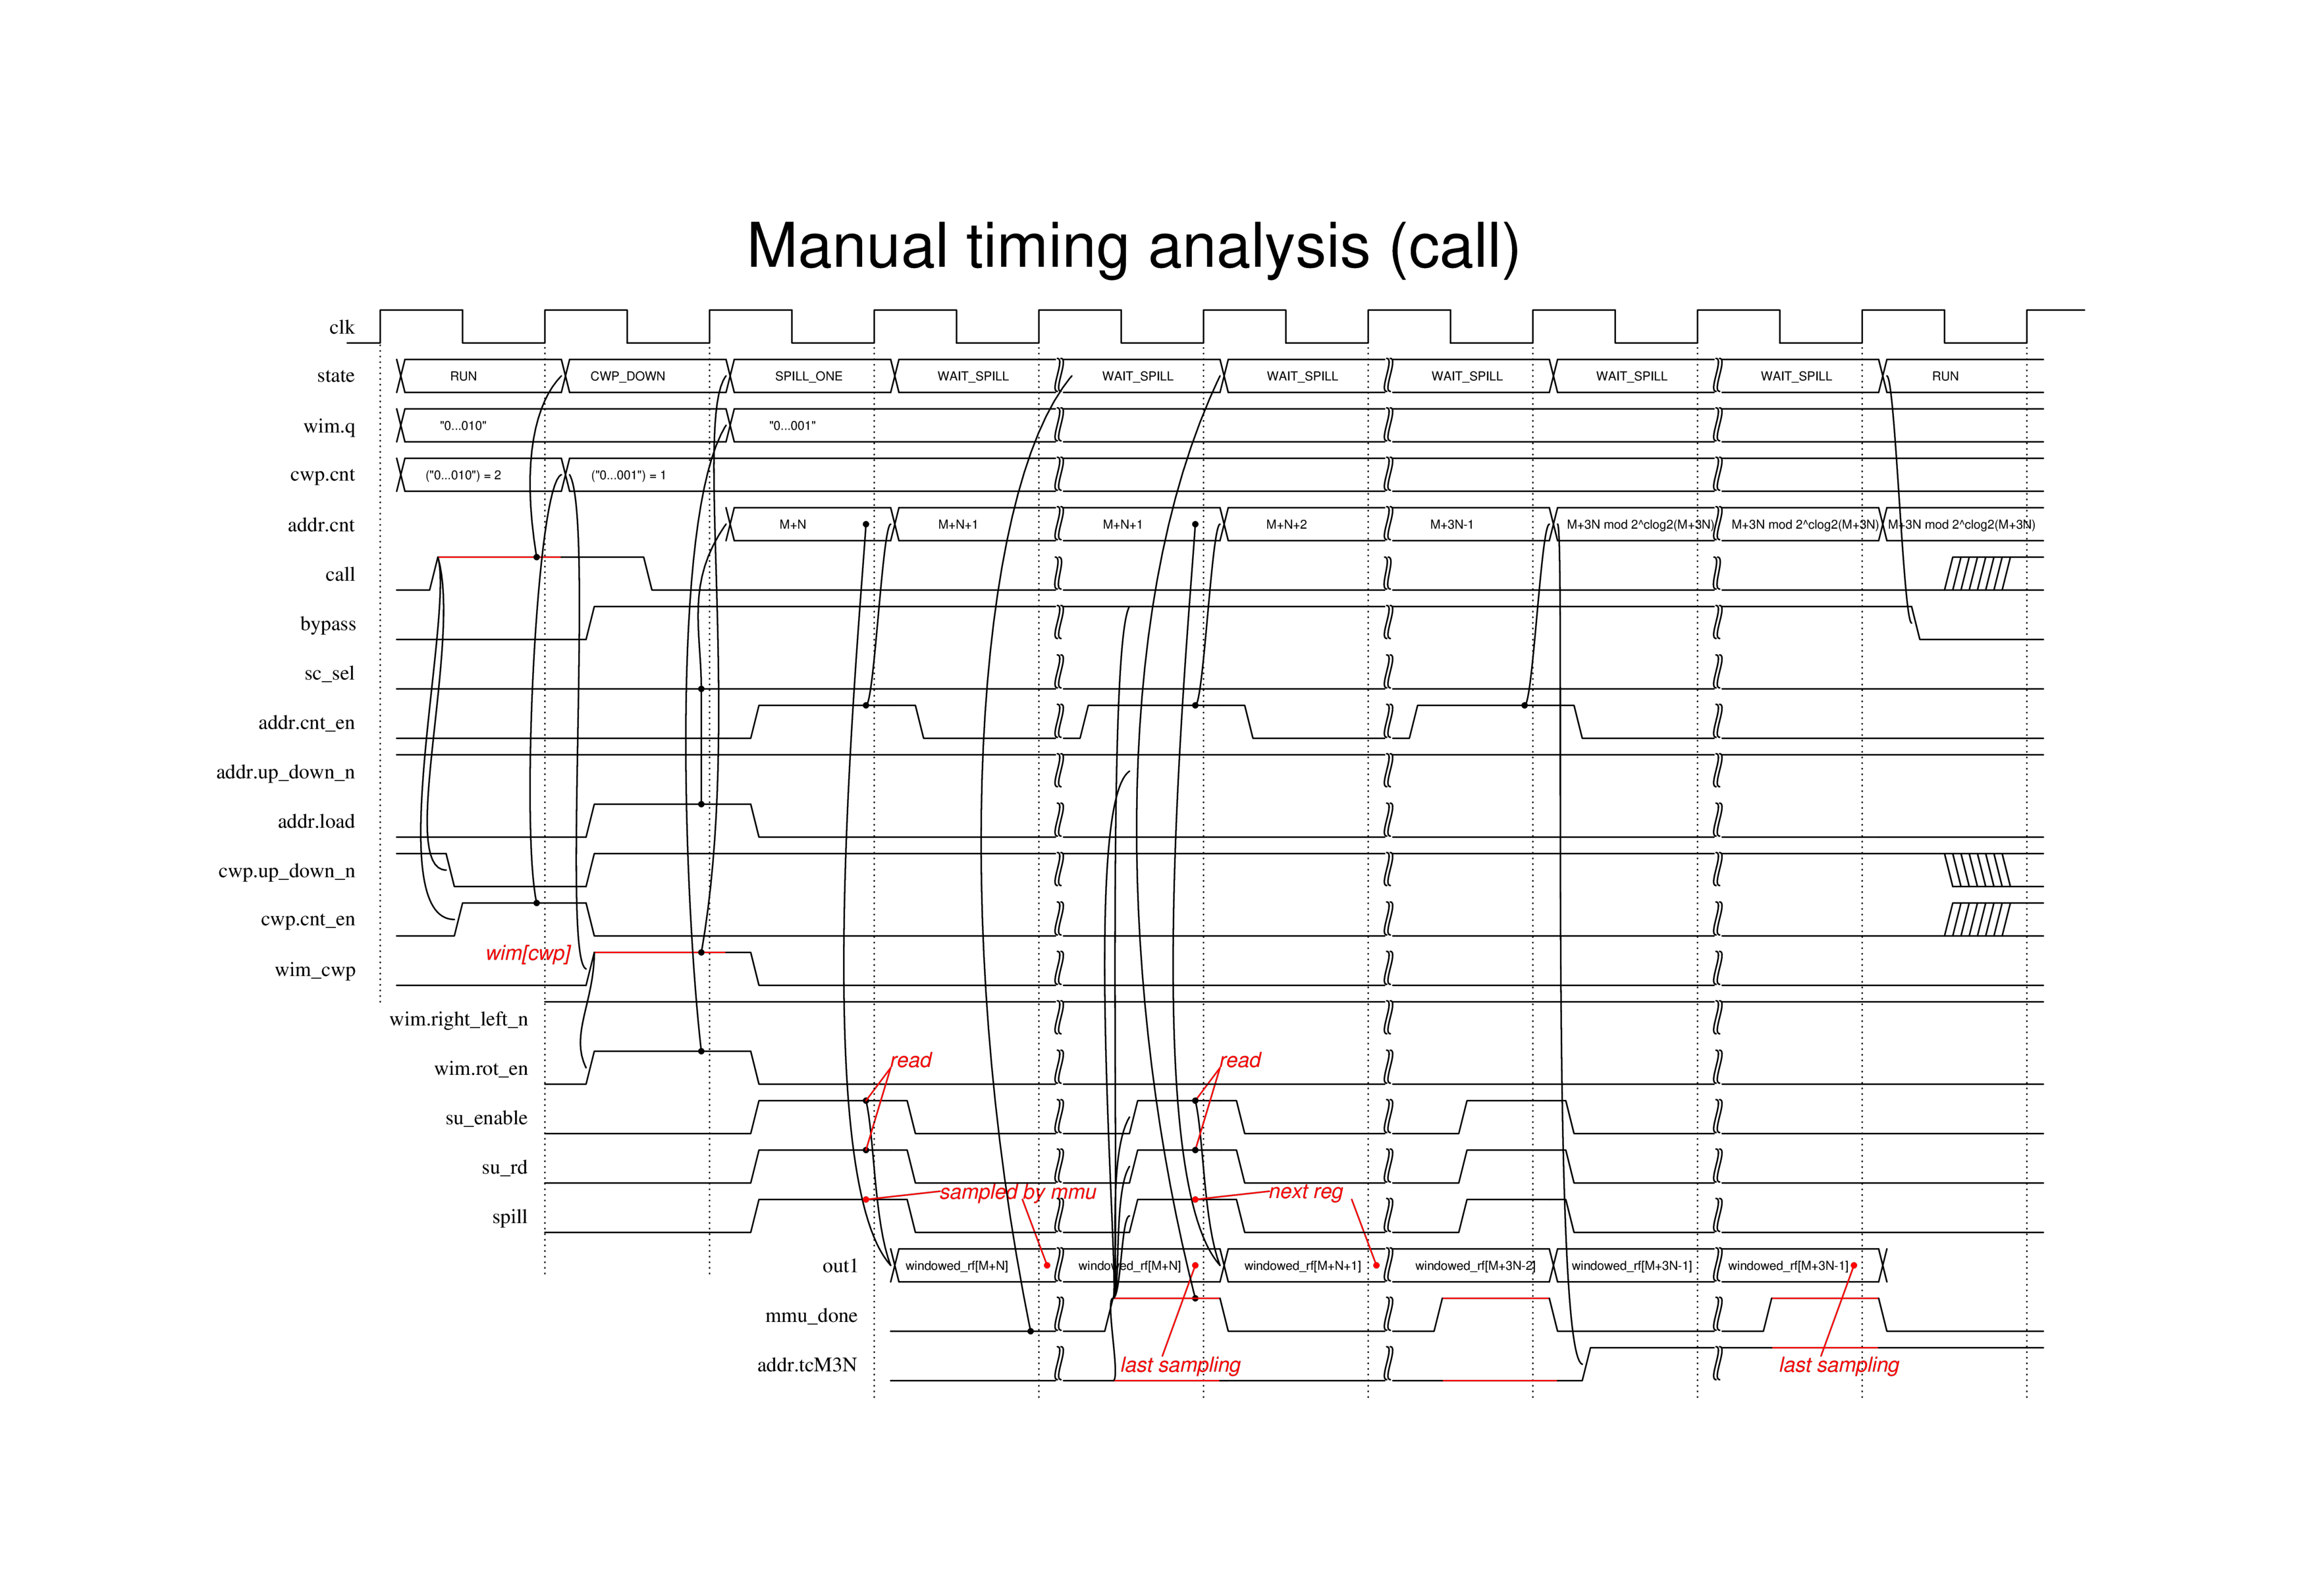
\includegraphics[width=\linewidth]{fig/windowed_rf/call_timing.pdf} \\
    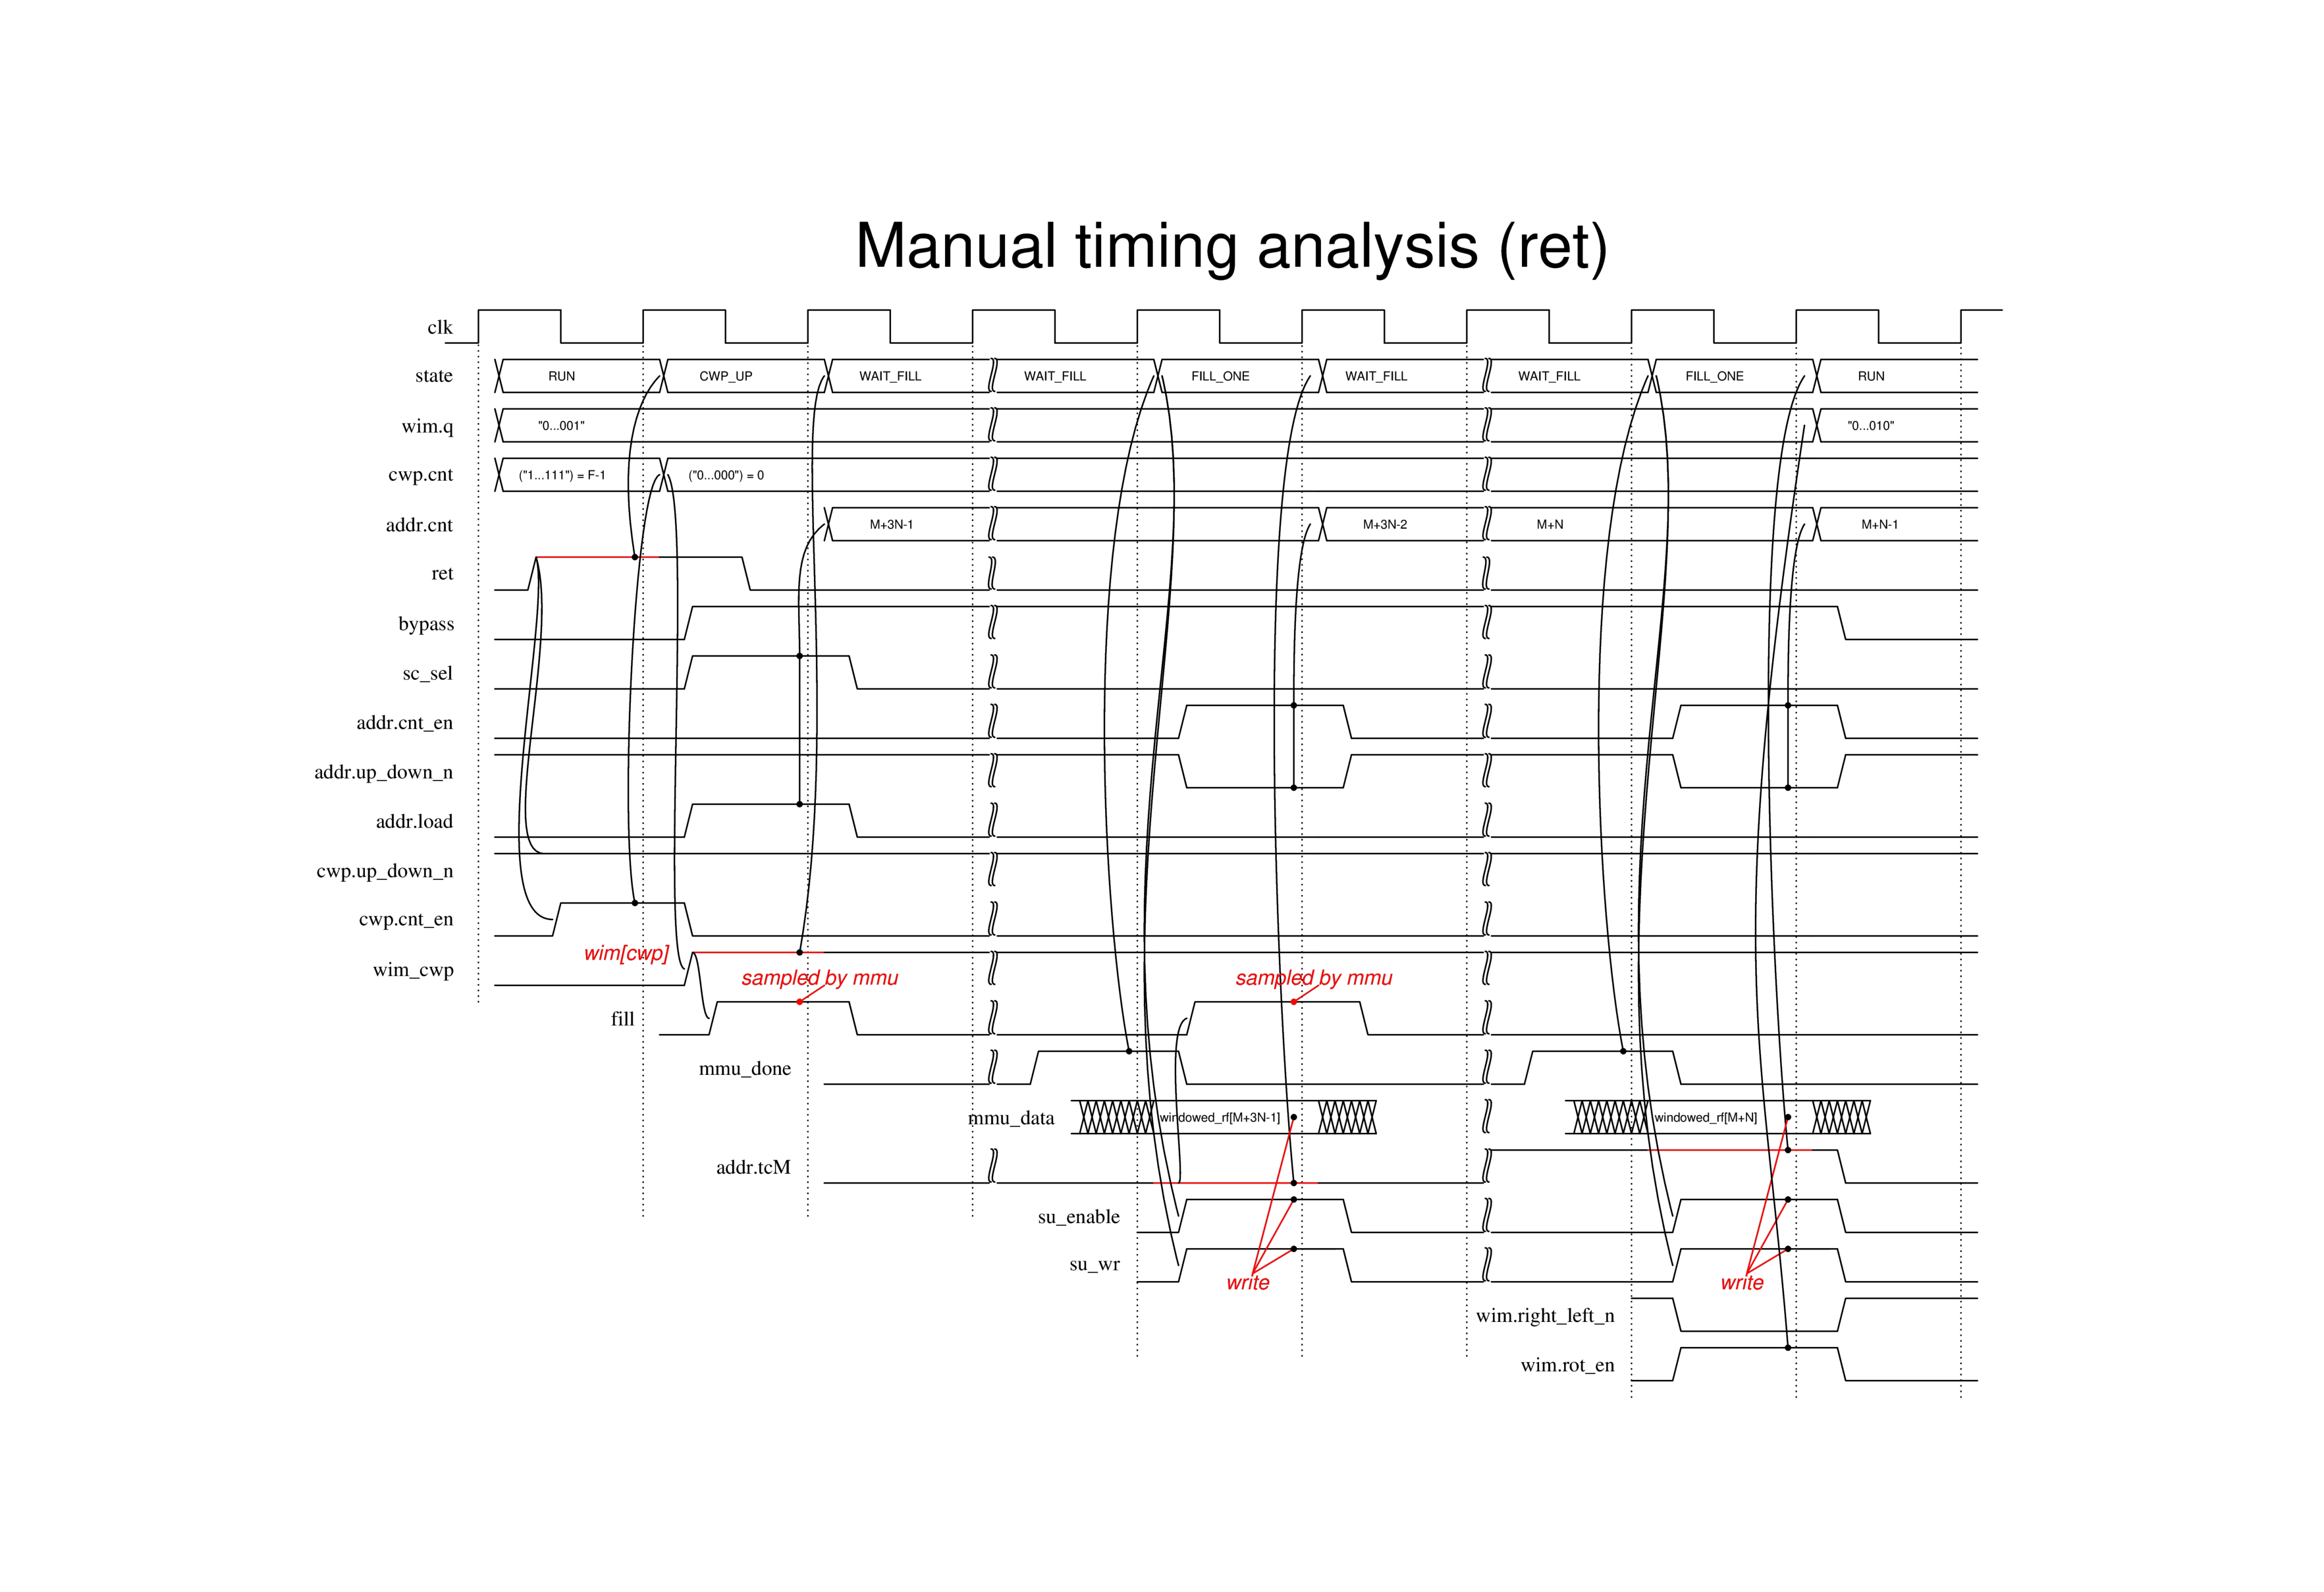
\includegraphics[width=\linewidth]{fig/windowed_rf/ret_timing.pdf}
    \caption{Timing details of call and return requests.}
    \label{fig:wrf_timing}
    \end{adjustwidth}
\end{figure}

\noindent What follows is the analysis of the \ac{uvm}-based verification of two intermediate designs from the \emph{Microelectronic Systems} course.
\begin{itemize}
    \item As an example of a combinational circuit, Intel's Pentium IV adder. According to the interface in~\cref{list:dut_p4}, it is designed both with generic parallelism and carry-generator tree sparseness.
    
    \item As a sequential circuit, the fixed-size windowed register file of~\cref{list:dut_wrf}, inspired by the SPARC instruction set architecture~\cite{SPARC:manv8}. The added difficulty of the overlapping windows organization is the management of call and return requests, whose control was designed according to the \ac{asm} methodology as shown in~\cref{fig:wrf_asm}. For the interaction with the memory management unit, a simple protocol was chosen; the detailed timing is in~\cref{fig:wrf_timing}.
    \begin{itemize}
        \item In the clock cycle after having sampled \vhdlinline{call} high, the \vhdlinline{bypass} signal is raised; if the call request triggers a spill operation, the \vhdlinline{spill} output is raised in the subsequent cycle and the spilled data becomes valid on \vhdlinline{out1} from the cycle onward. The memory management is expected to respond by raising the \vhdlinline{mmu_done} signal in the last clock cycle of data reading. 
        
        \item In the clock cycle after having sampled \vhdlinline{ret} high, the \vhdlinline{bypass} signal is raised; if the return triggers a fill operation, the \vhdlinline{fill} signal is also raised within the same cycle. The memory management unit recognizes the fill request by monitoring the \vhdlinline{fill} signal and responds by raising \vhdlinline{mmu_done} in the clock cycle before the data becomes valid on the \vhdlinline{mmu_data} input to the register file.
    \end{itemize}
    The reset is synchronous and prevails on call and return requests; in turn, the call request holds higher priority over the return. In the absence of these three, the \vhdlinline{enable} signal activates read and write operations, which must be further enabled port by port through the \vhdlinline{rd1}, \vhdlinline{rd2}, and \vhdlinline{wr} signals. In cases where the read and write addresses match, a read-before-write policy is adopted.
\end{itemize}